\documentclass{article}

\usepackage{graphicx}
\usepackage{tikz}
\usepackage{tikzsymbols}
\usetikzlibrary{calc,patterns,shapes.geometric}
\pagestyle{empty}
\usepackage[margin=0pt]{geometry}
\geometry{papersize={14in,12in}}

\def\centerarc[#1](#2)(#3:#4:#5){\draw[#1] ($(#2)+({#5*cos(#3)},{#5*sin(#3)})$) arc (#3:#4:#5);}

\begin{document}
	\begin{figure}
		\centering
		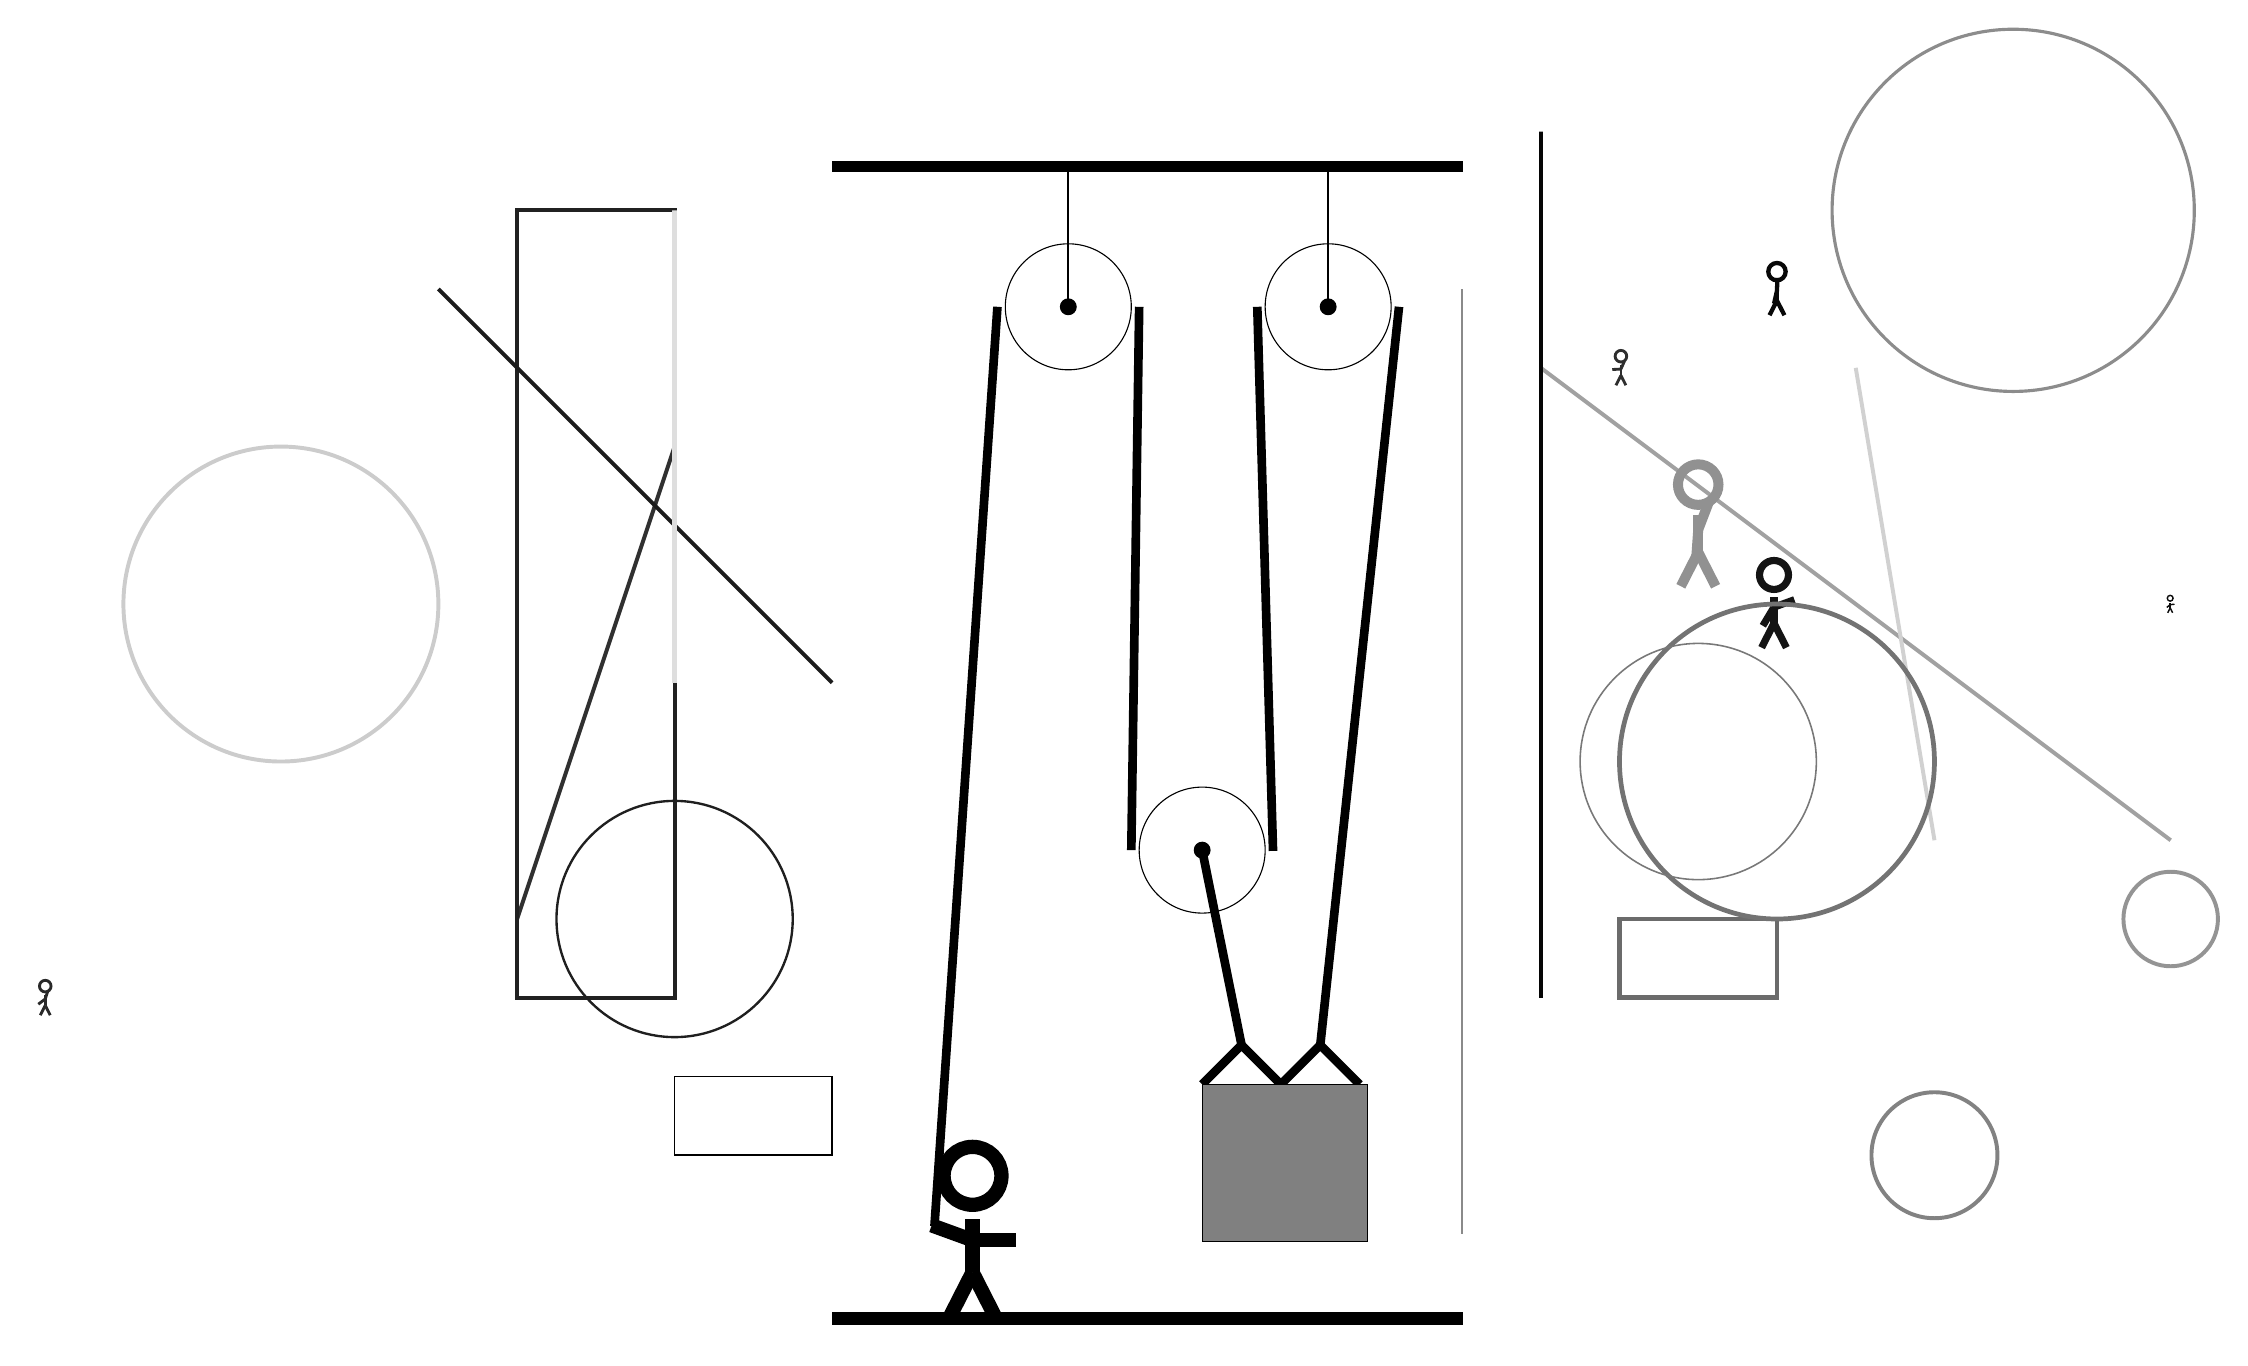
\begin{tikzpicture}
			%%%%% START %%%%%
			
			\draw[fill=black] (-2, 11.5) rectangle (6, 11.625);
			
			\draw (1, 9.775) circle (0.8);
			\draw[fill=black] (1, 9.775) circle (0.1);
			\draw[thick] (1, 9.775) -- (1, 11.5);
			
			\draw (4.3, 9.775) circle (0.8);
			\draw[fill=black] (4.3, 9.775) circle (0.1);
			\draw[thick] (4.3, 9.775) -- (4.3, 11.5);
			
			\draw (2.7, 2.875) circle (0.8);
			\draw[fill=black] (2.7, 2.875) circle (0.1);
			
			\draw[line width=1.1mm]  (2.7, -0.1) -- (3.2, 0.4) -- (3.7, -0.1) -- (4.2, 0.4) -- (4.7, -0.1);
			\draw[fill=black!50] (2.7, -0.1) rectangle (4.8, -2.1);
			
			\node[line width=0.2mm, color=black!95] at (15, 6) {\Strichmaxerl[1][39][6]};
			
			\node[line width=0.6mm, color=black!92] at (10, 6) {\Strichmaxerl[5][59][20]};
			\draw[line width=0.5mm, color=black!37](7, 9) -- (15, 3);
			\draw[line width=0.5mm, color=black!98] (7, 1) rectangle (7, 12);
			\draw[line width=0.5mm, color=black!81](-4, 8) -- (-6, 2);
			\draw[line width=0.3mm, color=black!46] (6, 10) rectangle (6, -2);
			
			\draw[line width=0.6mm, color=black!58] (8, 2) rectangle (10, 1);
			\node[line width=0.5mm, color=black!82] at (8, 9) {\Strichmaxerl[2][3][66]};
			\draw [line width=0.5mm, color=black!49](12, -1) circle (0.8);
			
			\draw[line width=0.5mm, color=black!87] (-4, 11) rectangle (-6, 1);
			
			\node[line width=0.5mm, color=black!43] at (9, 7) {\Strichmaxerl[7][86][69]};
			
			\draw [line width=0.5mm, color=black!42](15, 2) circle (0.6);
			\draw[line width=0.5mm, color=black!18](11, 9) -- (12, 3);
			\draw[line width=0.2mm, color=black!100] (-2, -1) rectangle (-4, 0);
			\draw [line width=0.6mm, color=black!55](10, 4) circle (2.0);
			\draw[line width=0.5mm, color=black!89](-2, 5) -- (-7, 10);
			
			\draw[line width=0.6mm, color=black!13] (-4, 11) rectangle (-4, 5);
			
			\node[line width=0.7mm, color=black!97] at (10, 10) {\Strichmaxerl[3][77][88]};
			\draw [line width=0.3mm, color=black!88](-4, 2) circle (1.5);
			\node[line width=0.7mm, color=black!84] at (-12, 1) {\Strichmaxerl[2][37][72]};
			\draw [line width=0.4mm, color=black!45](13, 11) circle (2.3);
			
			\draw [line width=0.5mm, color=black!20](-9, 6) circle (2.0);
			
			\draw [line width=0.2mm, color=black!53](9, 4) circle (1.5);
			
			\draw[line width=1.1mm](-0.7, -1.9) -- (0.1, 9.775);
			\centerarc[line width=1.1mm](1, 9.775)(0:180:0.9);
			\draw[line width=1.1mm](1.9, 9.775) -- (1.8, 2.875);
			\centerarc[line width=1.1mm](2.7, 2.875)(180:370:0.9);
			\draw[line width=1.1mm] (3.6, 2.865) -- (3.4, 9.775);
			\centerarc[line width=1.1mm](4.3, 9.775)(0:180:0.9);
			\draw[line width=1.1mm](4.2, 0.4) -- (5.2, 9.775);
			\draw[line width=1.1mm] (3.2, 0.4) -- (2.7, 2.875);
			
			\node at (-0.2, -2) {\Strichmaxerl[10][-20][0]};
			
			\draw[fill=black] (-2, -3) rectangle (6, -3.15);
			
			%%%%% END %%%%%
		\end{tikzpicture}
	\end{figure}	
\end{document}